\subsection{Passage throughflow}
As discussed in \fref{sec:throughflowp} the passage throughflow can be calculated using the velocity field for each time step. To do this a suitible location was chosen for each time step and passage such that there are no boundaries next to the passageways. This method is the same for each of the passages, noting that only zonal flow was studied. Thus we can study the effect of changes in bathymetry to on the relative strength of the flow.  The passageways have been labeled in figure (figure of these). The computed throughflow can be seen in \fref{fig:throughflow}. In this figure the onset of the ACC is clearly visible. Showing that due to the northward movement of Australia and the deepening of the drake passage the total volume transported by the ACC grows dramatically over time. Furthermore it can be seen that the closure of the drake passage causes the flow through the aghulas passage to reverse in direction. Furthermore, the throughflow through the panama passage is shown to slow due to both the onset of the ACC and the closure of the thetys seaway. Finally reversing the direction of flow through the panama passage at 15Ma due to the total closure of the thetys sea. The reversal of the Indonesian throughflow observed by \cite{Mulder2017Jul} is not observed with total throughflow always moving water east to west. This is however in agreement to the flow found by \cite{omta2003physical} in a shallow water model. Note however, that the land masks used by them are different to the land masks used in this paper.

\begin{figure}[H]
	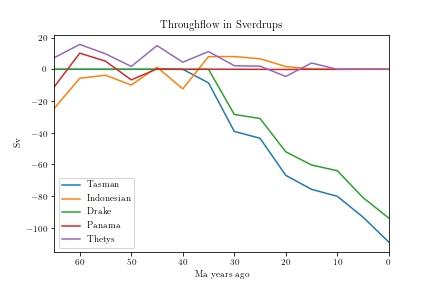
\includegraphics[width=\linewidth]{throughflow}
	\caption{Total volume transport in Sverdups for 7 passages. Running from 65 milion years ago to the present day situation. Positive values indicate transport to the west}
	\label{fig:throughflow}
\end{figure}

Rather than looking only at volume transport in the upper layers the transport can also be split into a deep water transport layer ($<-2000m$) and a surface transport layer($>-2000m$). Doing this gives insight into the thermohaline circulation. In the deep water transport layer seen in \fref{fig:throughflow_bottom} we see a very diffirent picture to the total volume transport. It is however hard to draw any conclusions from this image. It is only 6 integration layers deep and fluctuations in the depth of each passage accounts for most of the differences comparing each time step.

(THIS NEEDS MORE SIMULATION TIME)
\begin{figure}[H]
	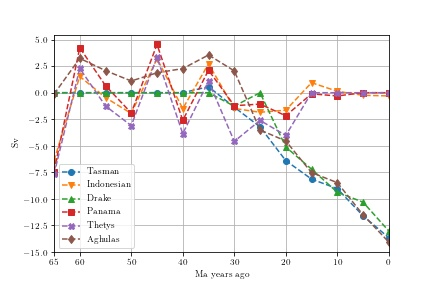
\includegraphics[width=\linewidth]{throughflow_deep_0_6}
	\caption{Total volume transport in the deep water layer ($<-2000m$) in Sverdups for 7 passages. Running from 65 milion years ago to the present day situation. Positive values indicate transport to the west}
	\label{fig:throughflow_bottom}
\end{figure}


To get an even better understanding of the flows, we can look at a vector field showing the direction of horizontal water displacement for each of the time steps. This is done by making a weighted mean of the horizontal flow field for each layer. Weighted by the volume of each grid cell. In this way each arrow actually represents relative flow velocity compared to other grid points. Thus showing the velocity field of the ocean. 

This field is shown in \fref{fig:flowfield}. Here the ACC is very noticible. The reversal of flow through the panama passage at $15Ma$ is the most interesting result here.  Where here we find the closure of the Thetys seaway to be the main factor. However, the reversal only occurs after the closure of the seaway. This is in contrast to the results obtained by \cite{omta2003physical} where the flow reversal was observed to coincide with the opening of the drake passage. Here we only observe a decease in volume transported through the passage, but no such reversal until the Thetys seaway is closed.

The largest changes in the flow field are observed in the Indian ocean. The indian continent moves northward at a very fast pace. After 55 Ma the flow through the passage north of the Indian continent is massively reduced and instead the water flows east of the continent into the thetys seaway. No "circum India" current is observed in any of the time steps. The position of the Indian continent does however seem to have a strong influence on the strength of the Aghulas sub-tropical gyre. This can probably be explained by the amount of water that is transported through the Tethys seaway. There being a large fluctuation in the strength of the gyre. The size of this gyre also increases with time due to this northward movement.
